\begin{mainquestion}{diodepullup}{Diode-Connected Load Common-Source Amplifier}

\questionpoints

The figure below shows a diode-connected transistor used as a replacement for the pull-up resistor in a common-source (CS) amplifier.

\begin{center}
    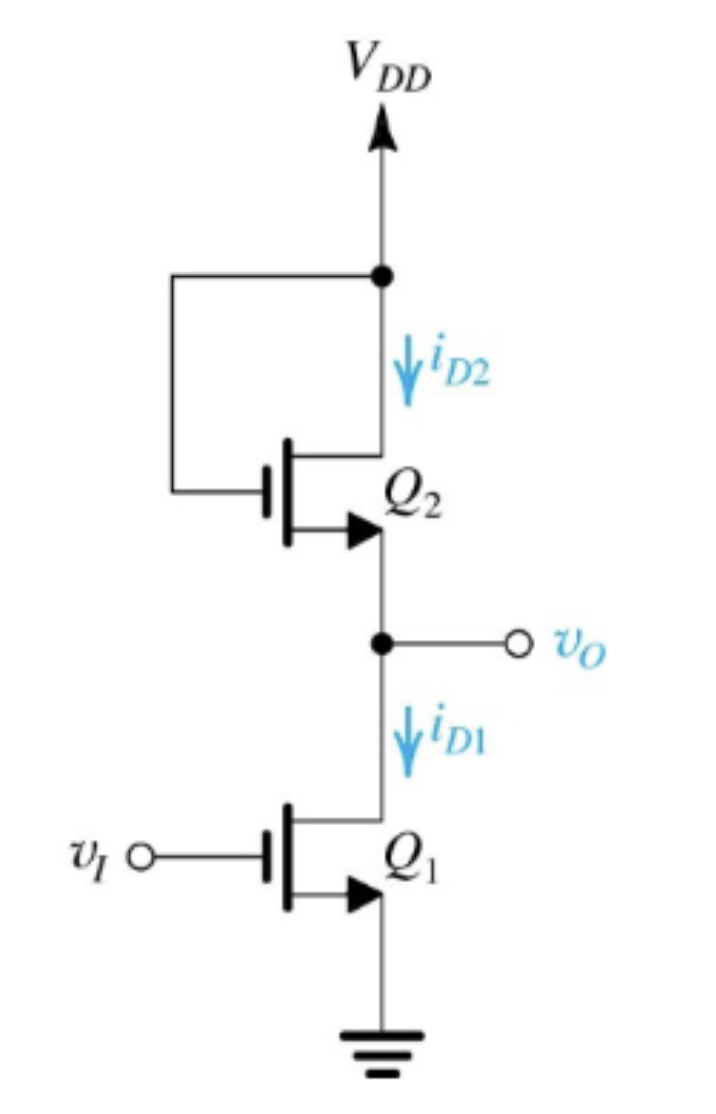
\includegraphics[width=0.3\textwidth]{q3.png}
\end{center}

%------------------------------------------------

% =========================================================
\begin{partquestion}{deriveoutput}
{Assume both transistors are in saturation. Show that the output voltage is

\[
v_o = V_{DD} - V_t 
+ \sqrt{\frac{(W/L)_1}{(W/L)_2}}\,V_t 
- \sqrt{\frac{(W/L)_1}{(W/L)_2}}\,v_i
\]

assuming that both transistors have the same threshold voltage $V_t$.  

Thus, the circuit functions as a linear amplifier even for large input signals.}

\begin{answer}
When both transistors are in saturation, the drain currents are equal:

\[
i_{D1} = i_{D2}.
\]

Using the saturation current expression:

\[
\frac{1}{2} k' \left(\frac{W}{L}\right)_1 (v_i - V_t)^2
=
\frac{1}{2} k' \left(\frac{W}{L}\right)_2 (V_{DD} - v_o - V_t)^2.
\]

Canceling $\frac{1}{2}k'$:

\[
\left(\frac{W}{L}\right)_1 (v_i - V_t)^2
=
\left(\frac{W}{L}\right)_2 (V_{DD} - v_o - V_t)^2.
\]

Taking square roots:

\[
\sqrt{\frac{(W/L)_1}{(W/L)_2}} (v_i - V_t)
=
V_{DD} - v_o - V_t.
\]

Solving for $v_o$:

\[
v_o
=
V_{DD} - V_t
+
\sqrt{\frac{(W/L)_1}{(W/L)_2}} V_t
-
\sqrt{\frac{(W/L)_1}{(W/L)_2}} v_i.
\]

This expression is linear in $v_i$, so the circuit behaves as a linear amplifier even for large input signals.
\end{answer}

%------------------------------------------------
\end{partquestion}

% =========================================================
\begin{partquestion}{saturationrange}
{Using the result above, determine the range of $v_i$ over which $Q_1$ is in saturation.}

\begin{answer}
For $Q_1$ (NMOS) to be in saturation:

\[
V_{GS1} > V_t
\quad \text{and} \quad
V_{DS1} \ge V_{GS1} - V_t.
\]

Since

\[
V_{GS1} = v_i, 
\qquad
V_{DS1} = v_o,
\]

the conditions become

\[
v_i > V_t,
\]
\[
v_o \ge v_i - V_t.
\]

Substituting the expression for $v_o$:

\[
V_{DD} - V_t
+ \sqrt{\frac{(W/L)_1}{(W/L)_2}} V_t
- \sqrt{\frac{(W/L)_1}{(W/L)_2}} v_i
\ge
v_i - V_t.
\]

Solving for $v_i$:

\[
v_i
\le
\frac{
V_{DD}
+
\sqrt{\frac{(W/L)_1}{(W/L)_2}} V_t
}{
1 + \sqrt{\frac{(W/L)_1}{(W/L)_2}}
}.
\]

Therefore, $Q_1$ remains in saturation for

\[
\boxed{
V_t
<
v_i
<
\frac{
V_{DD}
+
\sqrt{\frac{(W/L)_1}{(W/L)_2}} V_t
}{
1 + \sqrt{\frac{(W/L)_1}{(W/L)_2}}
}.
}
\]
\end{answer}

\pagebreak
%------------------------------------------------
\end{partquestion}

% =========================================================
\begin{partquestion}{gaincalc}
{Find the voltage gain for 
\[
W_1 = 10\,\mu m, \quad 
W_2 = 1\,\mu m, \quad 
L_1 = L_2 = 0.2\,\mu m.
\]

Given that $L$ is often constrained for a given technology, describe a potential approach to increasing the gain for this amplifier configuration.}

\begin{answer}
The voltage gain is

\[
A_v = \frac{d v_o}{d v_i}
=
- \sqrt{\frac{(W/L)_1}{(W/L)_2}}.
\]

Since $L_1 = L_2$,

\[
A_v
=
- \sqrt{\frac{W_1}{W_2}}
=
- \sqrt{\frac{10}{1}}
=
- \sqrt{10}
\approx -3.16.
\]

To increase the gain magnitude (with fixed $L$), we must increase the ratio

\[
\frac{(W/L)_1}{(W/L)_2}.
\]

Since $L$ is technology-constrained, this can be achieved by increasing $W_1$ or decreasing $W_2$.
\end{answer}

\end{partquestion}

\end{mainquestion}
